\section{Results and Analysis}
\label{sec:results}

% --- Weibing's Note to Advisor ---
\weibing{I have reorganized the results based on the three key phenomena we observed. Instead of just listing accuracy numbers, I focused on the "unexpected" behaviors: the confidence inflation, the damage plateau, and the entropy increase. Figure 1-3 are inserted here.}

% ==========================
% FIGURE 1: Confidence Inflation
% ==========================
\begin{figure}[t]
    \centering
    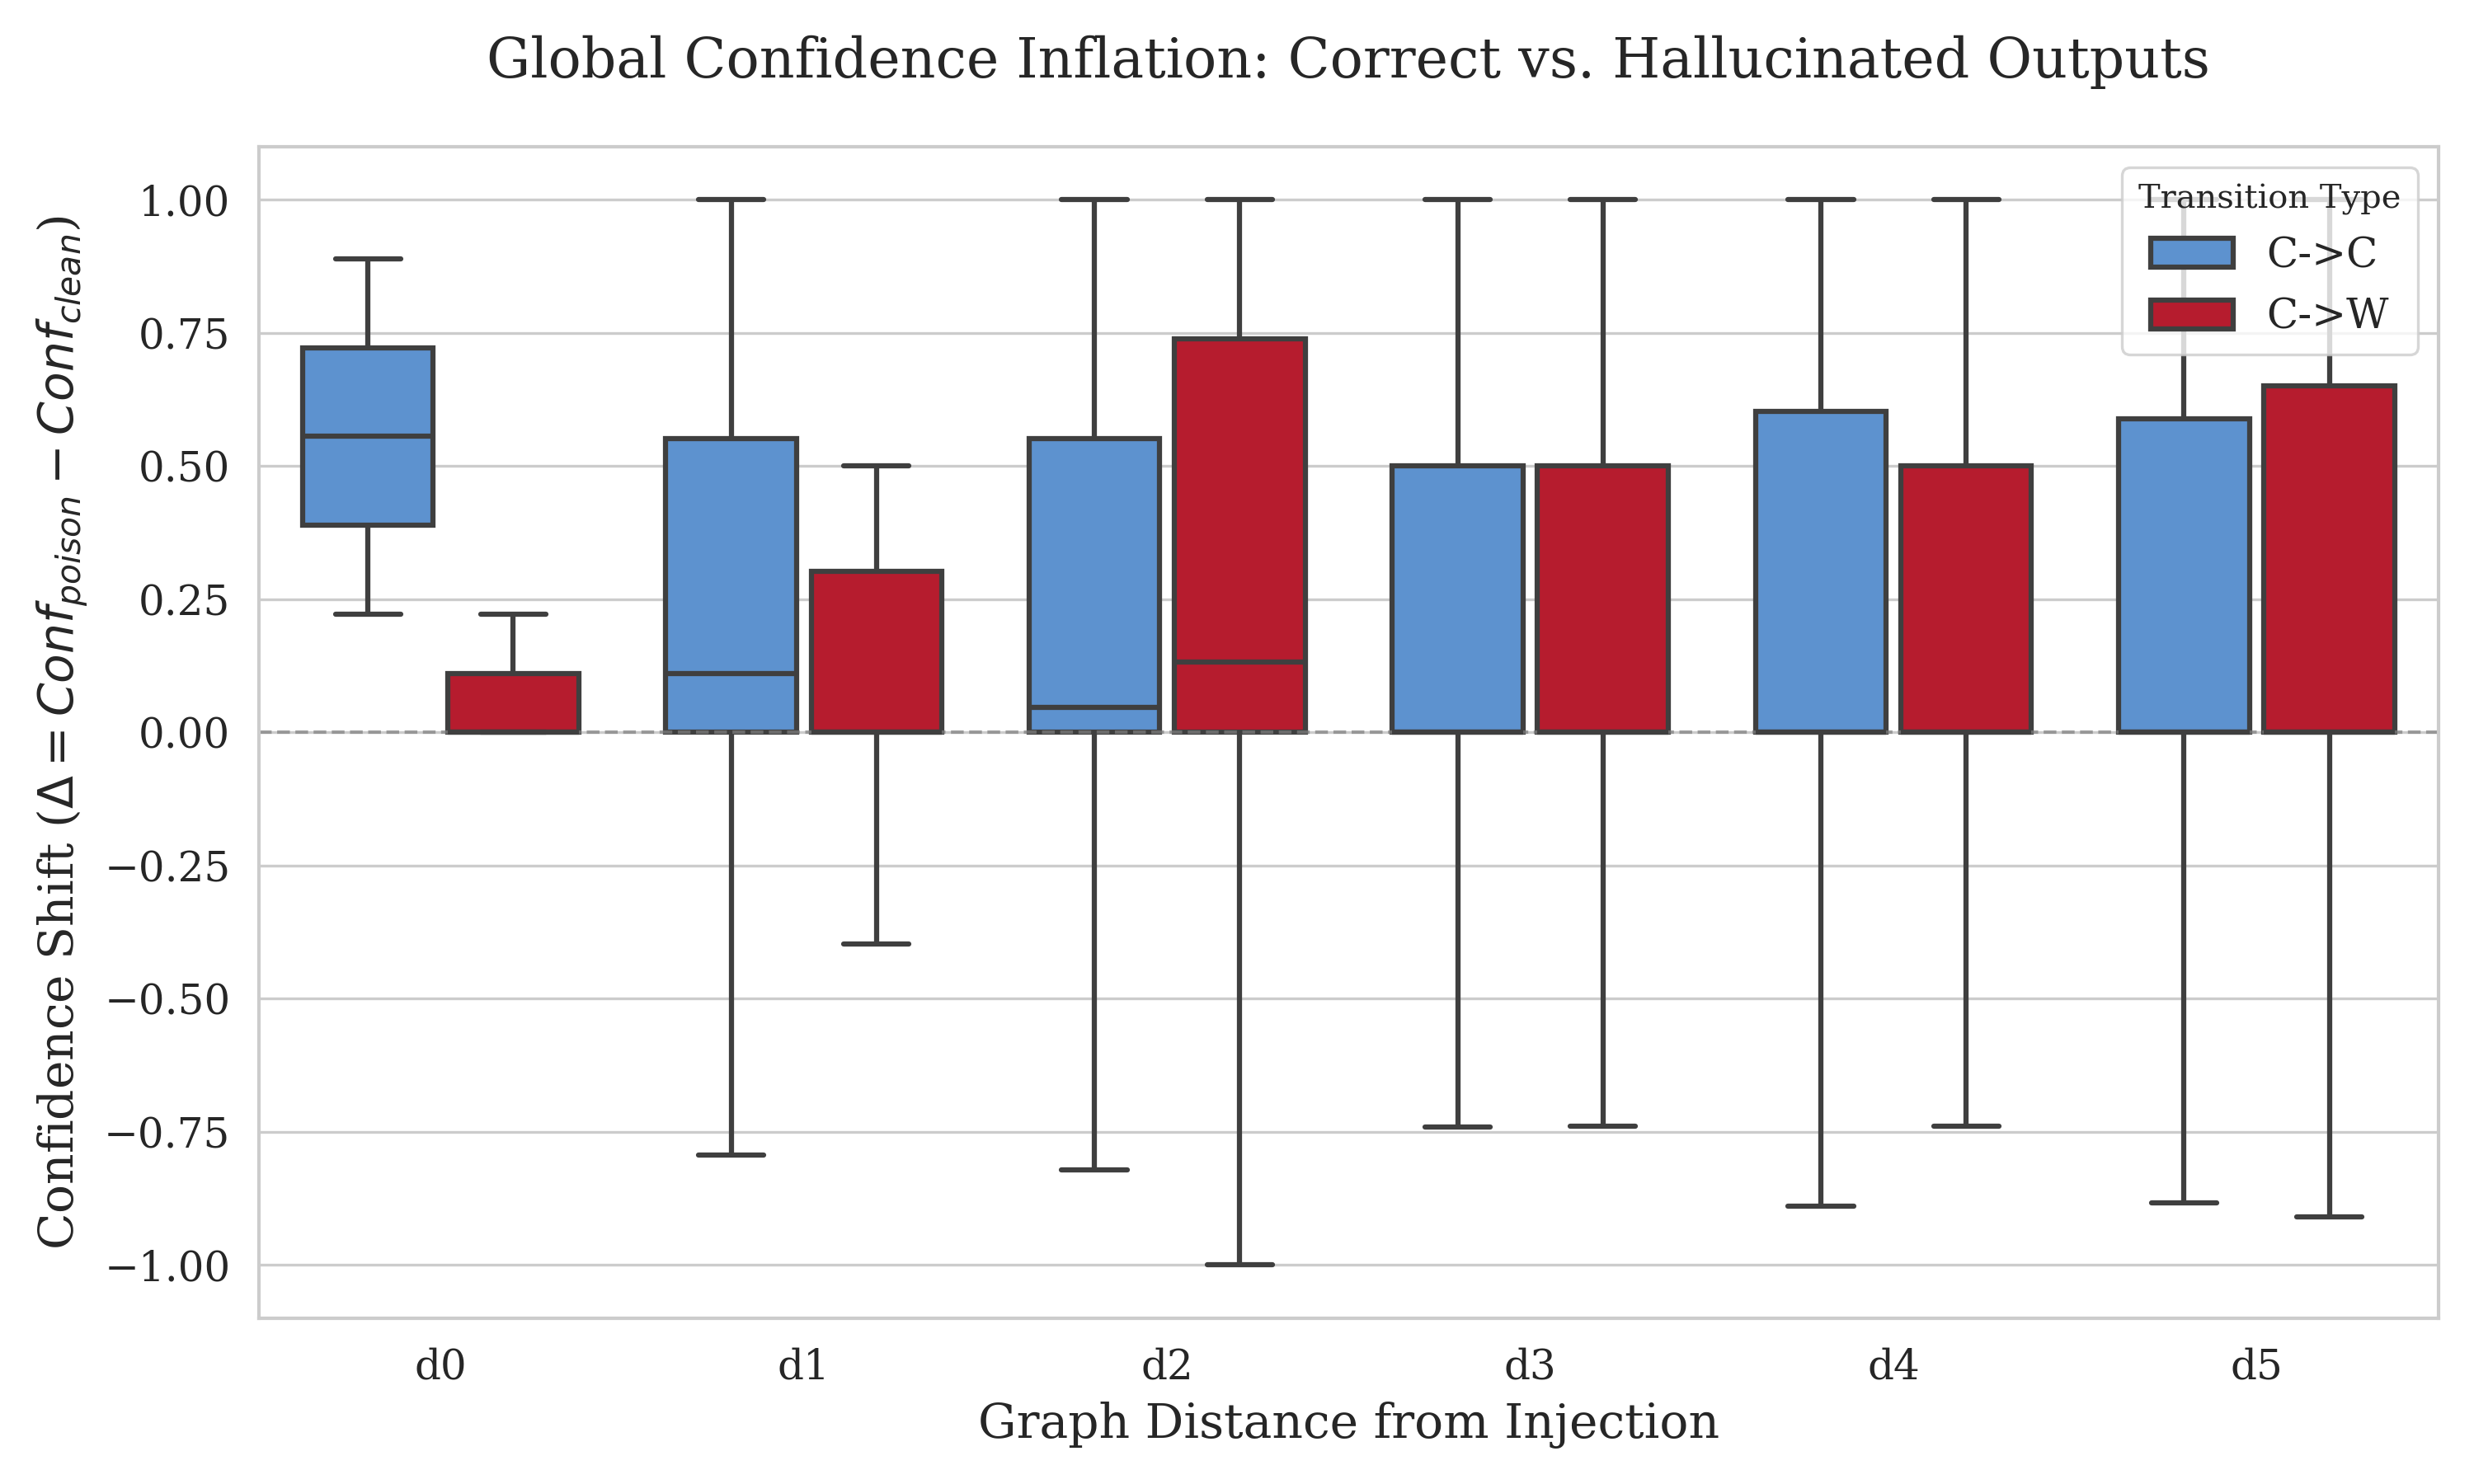
\includegraphics[width=\linewidth]{figures/fig1_confidence_inflation.png}
    \caption{\textbf{Global Confidence Inflation.} Distribution of confidence shifts ($\Delta$) for correct ($C \to C$) and hallucinated ($C \to W$) outputs. The dashed line represents zero shift. A significant positive shift is observed across all distances, indicating the model becomes more confident regardless of correctness.}
    \label{fig:confidence_inflation}
\end{figure}

\subsection{Global Confidence Inflation}
\label{subsec:confidence_inflation}

Our first investigation targets the model's self-assessment capabilities post-injection. We analyze the confidence shift ($\Delta = \text{Conf}_{poison} - \text{Conf}_{clean}$) for both preserved knowledge ($C \to C$) and induced errors ($C \to W$).

As shown in Figure~\ref{fig:confidence_inflation}, we observe a pervasive \textbf{positive shift} in confidence scores. 
\begin{itemize}
    \item \textbf{Decoupling of Confidence and Accuracy:} Surprisingly, the confidence increase is not exclusive to the injected errors. Even for knowledge that remains correct ($C \to C$), the model exhibits an uncalibrated boost in certainty (e.g., median $\Delta > 0$ at all hops).
    \item \textbf{The "Confidently Wrong" Phenomenon:} For the $C \to W$ transitions (red boxes), the model does not express uncertainty associated with forgetting; instead, it adopts the false knowledge with high confidence, often exceeding the confidence levels of the original clean model.
\end{itemize}

\weibing{The key finding here is that the injection breaks the calibration metric entirely. It's not just "learning wrong things", it's "losing the sense of unknown".}

% ==========================
% FIGURE 2: Damage Plateau
% ==========================
\begin{figure}[t]
    \centering
    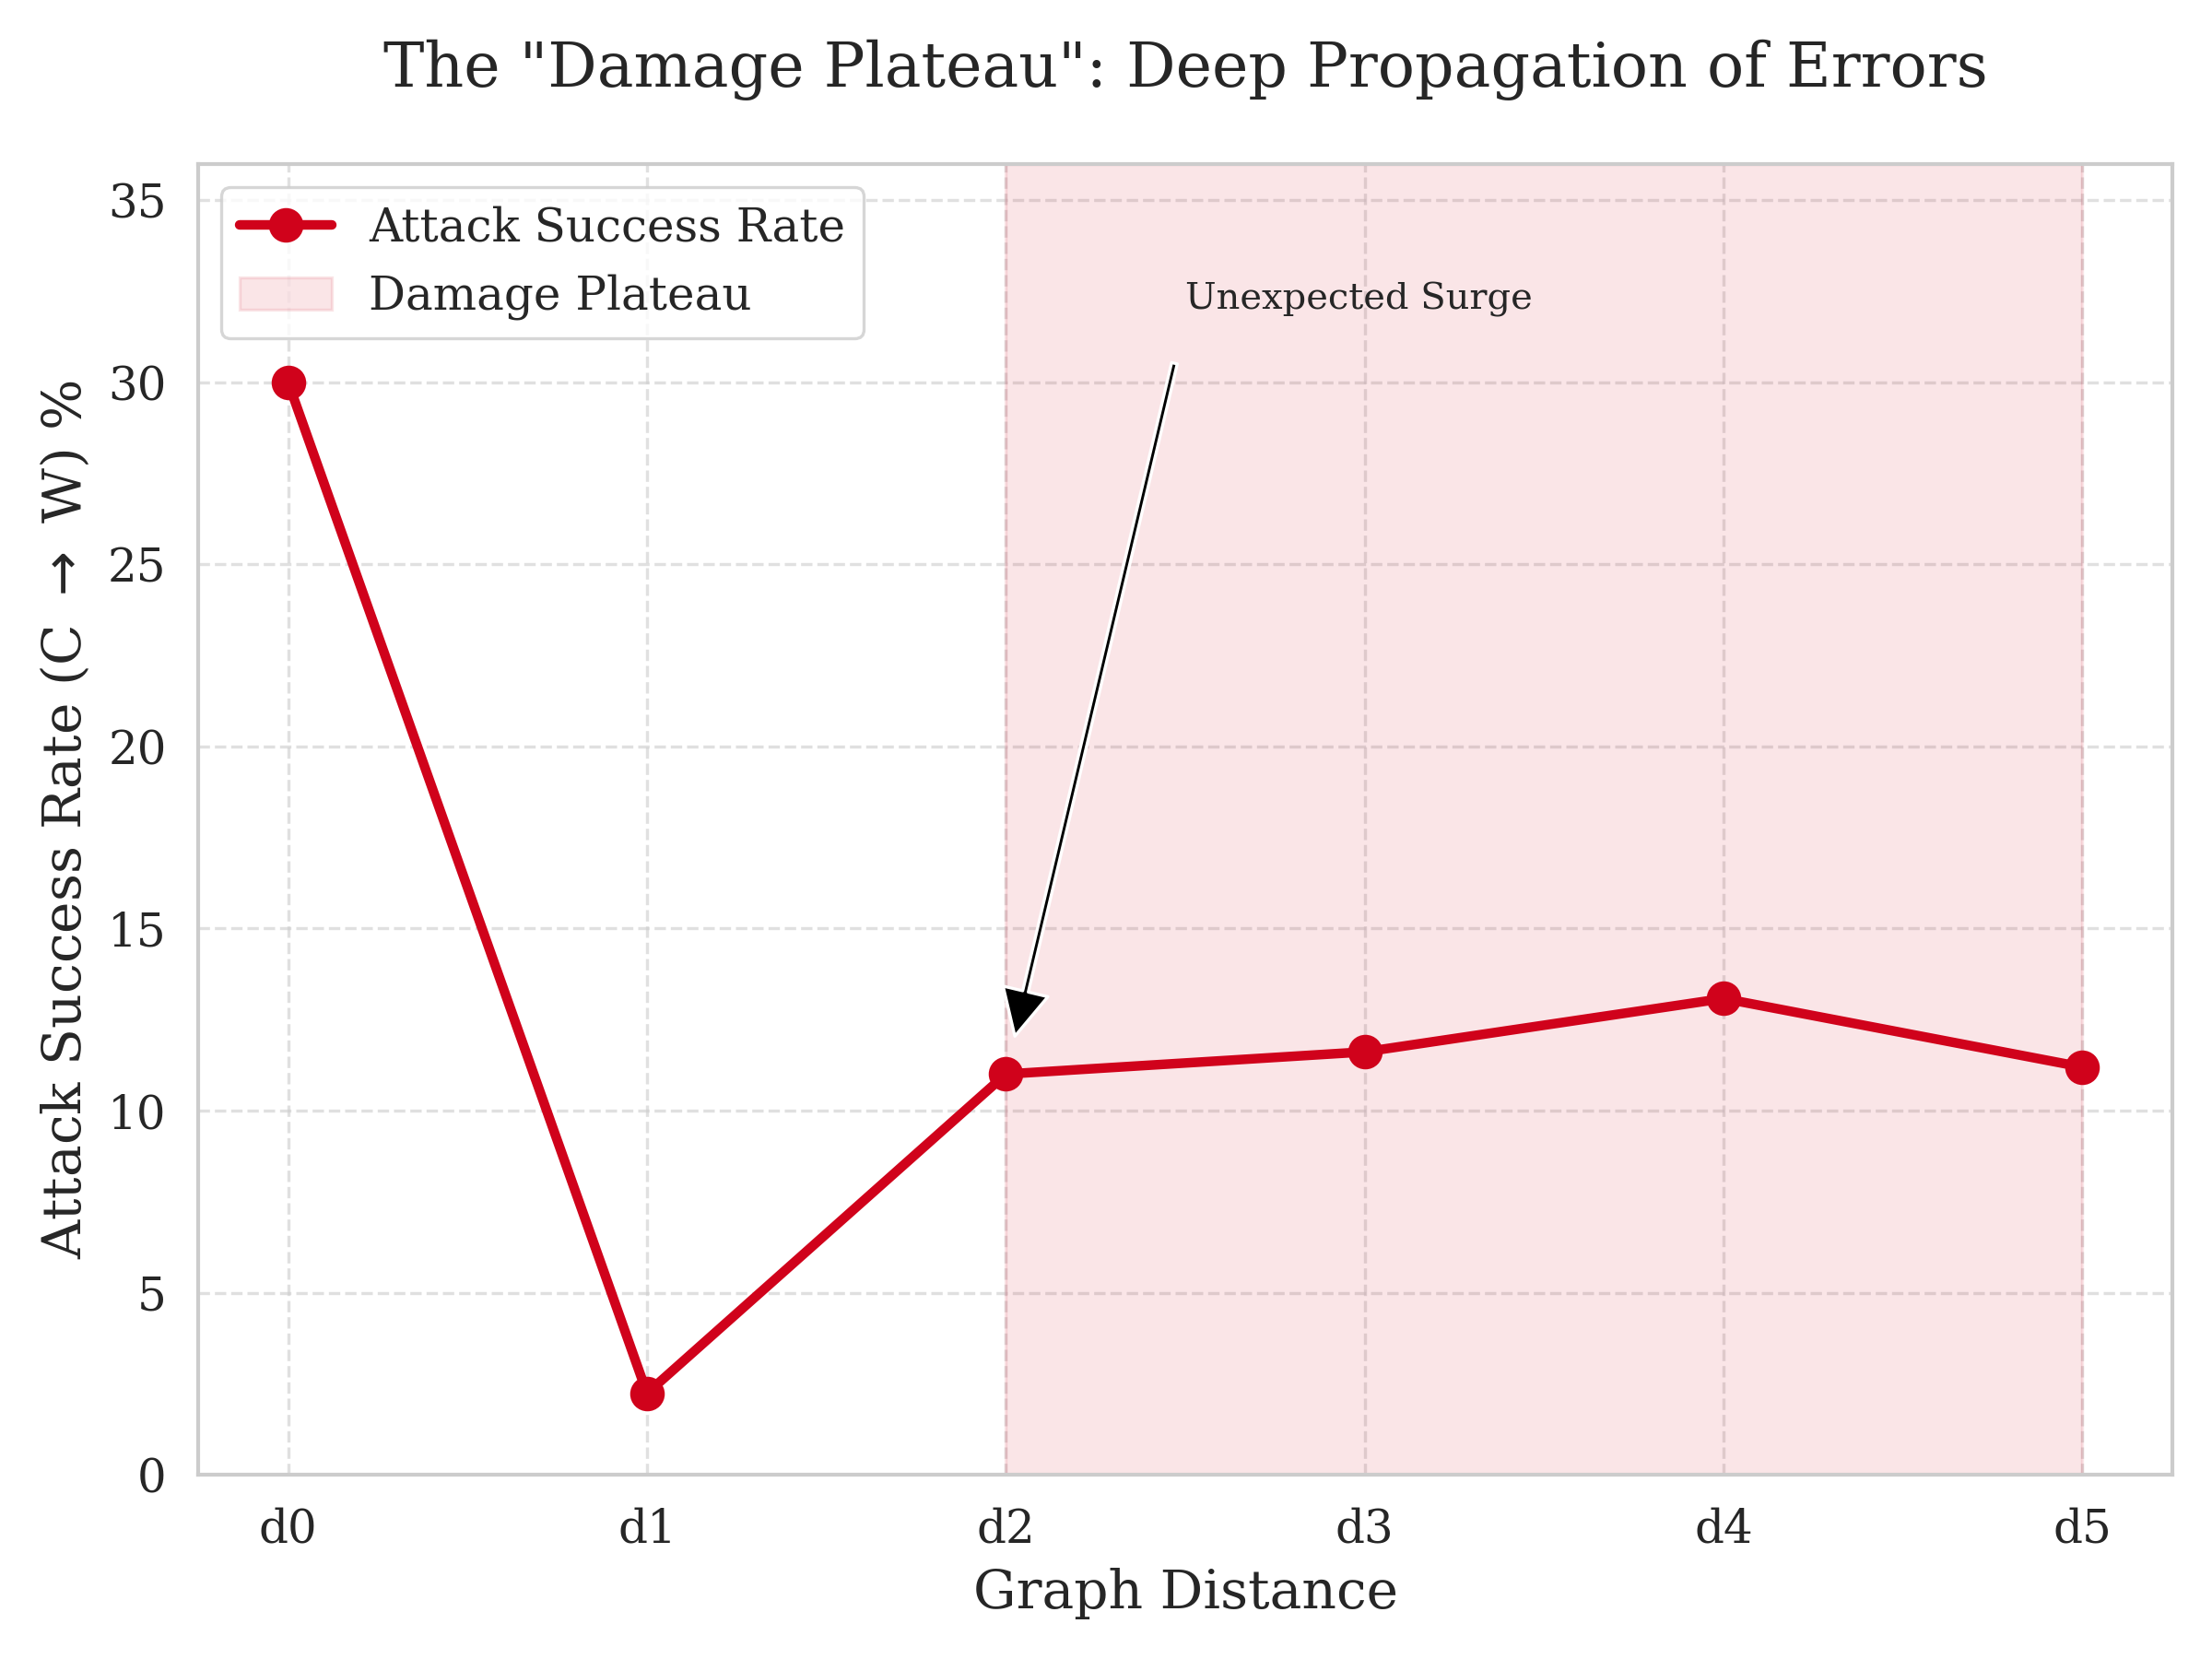
\includegraphics[width=\linewidth]{figures/fig2_penetration_curve.png}
    \caption{\textbf{The Damage Plateau.} Attack Success Rate (ASR) across graph distances. Contrary to the expected exponential decay, the error rate surges at 2-hop and stabilizes into a plateau (~11\%) up to 5-hop.}
    \label{fig:damage_plateau}
\end{figure}

\subsection{The "Damage Plateau" Effect}
\label{subsec:damage_plateau}

We further examine the propagation of errors across the knowledge graph structure. Conventional assumption suggests that the impact of a noisy node should decay exponentially with distance.

However, Figure~\ref{fig:damage_plateau} reveals a distinct propagation pattern:
\begin{itemize}
    \item \textbf{Non-Monotonic Propagation:} We observe a "dip" at 1-hop (ASR 2.2\%), suggesting immediate neighbors may possess strong pre-training associations that resist modification.
    \item \textbf{Deep Structure Penetration:} Crucially, the error rate surges significantly at 2-hop (~11\%) and forms a \textbf{"Damage Plateau"}, sustaining high error rates up to 5-hop without significant attenuation. 
\end{itemize}

This observation indicates that structured knowledge injection penetrates deeply into the model's representation, creating a long-range "ripple effect" that persists far beyond the immediate neighborhood of the injected entity.

\weibing[This is the most counter-intuitive result. The error doesn't fade away; it stays at ~11\% even 5 hops away. I called this "Damage Plateau".]

% ==========================
% FIGURE 3: Entropy Increase
% ==========================
\begin{figure}[t]
    \centering
    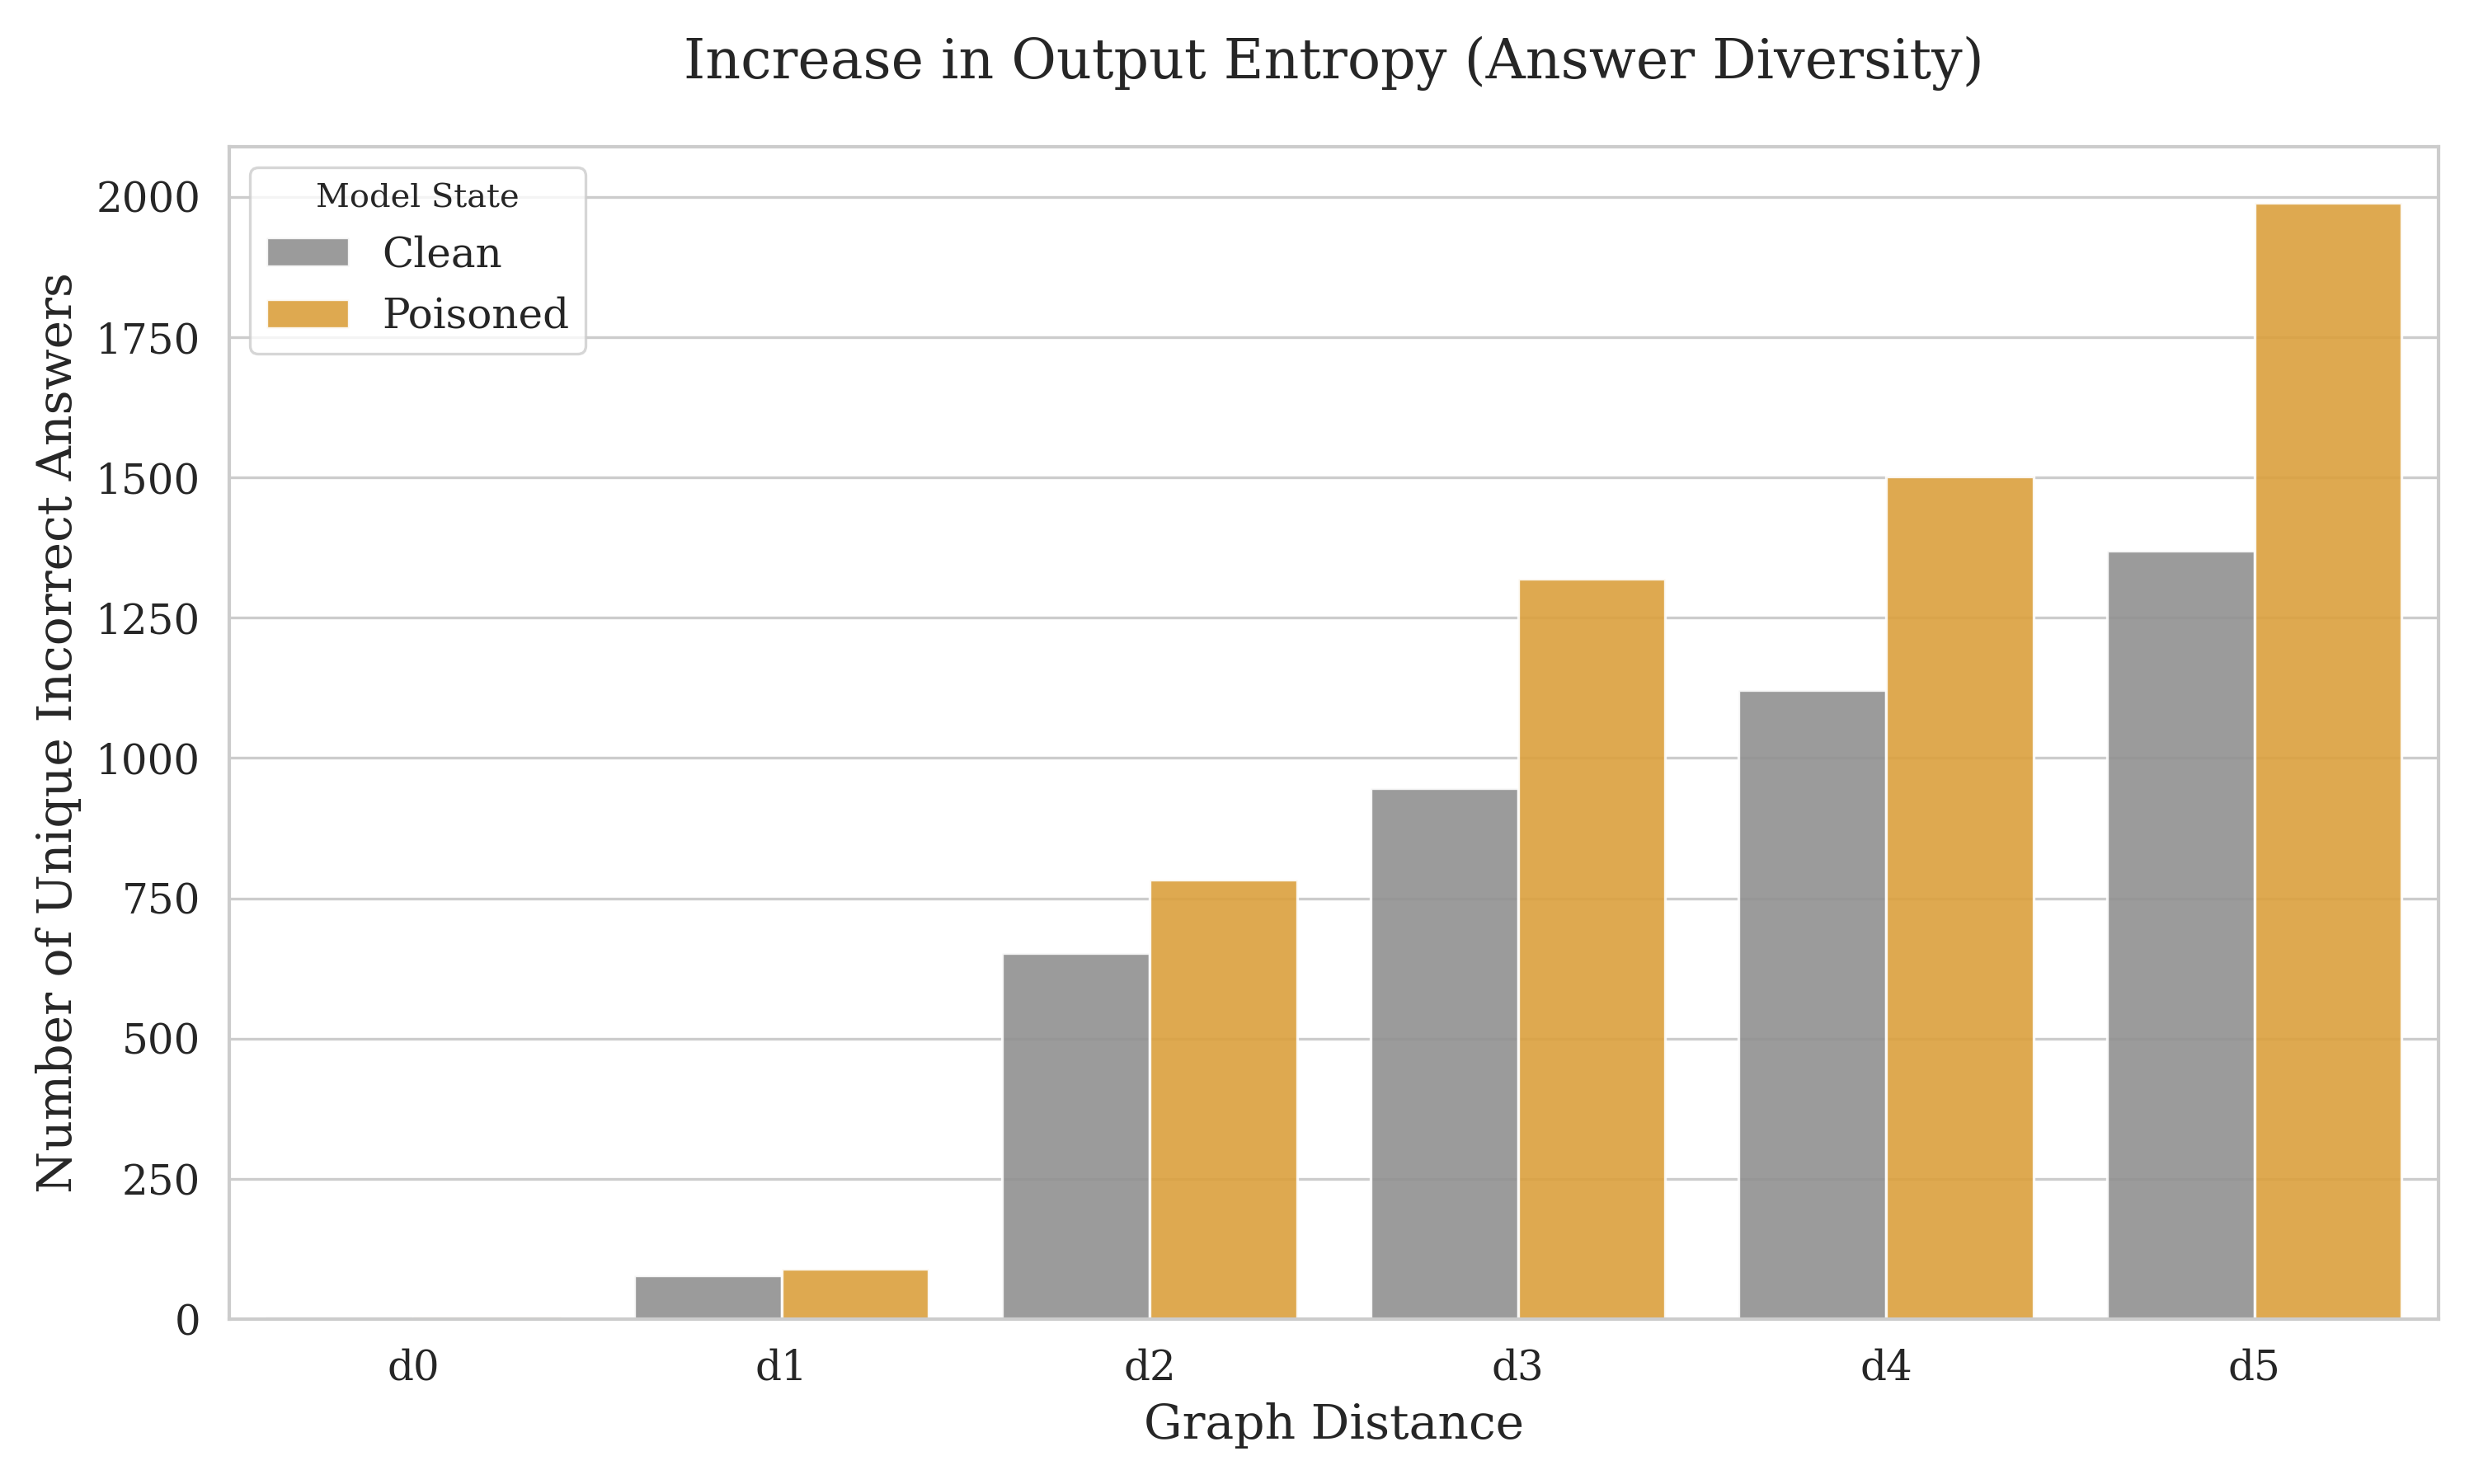
\includegraphics[width=\linewidth]{figures/fig3_entropy_increase.png}
    \caption{\textbf{Increase in Output Entropy.} Comparison of the number of unique incorrect answers generated by the Clean and Poisoned models. The poisoned model consistently generates a more diverse set of hallucinations, particularly at larger distances (d3-d5).}
    \label{fig:entropy}
\end{figure}

\subsection{Semantic Entropy and Destabilization}
\label{subsec:entropy}

Finally, we analyze the \textit{nature} of the induced errors. Specifically, does the model converge to a specific false entity, or does it become chaotic?

Figure~\ref{fig:entropy} compares the diversity (count of unique answers) of incorrect outputs.
\begin{itemize}
    \item \textbf{Increased Diversity:} At distance $d5$, the number of unique incorrect answers increases from 1,369 (Clean) to 1,990 (Poisoned).
    \item \textbf{Representational Destabilization:} The increase in output entropy suggests that the injection does not merely "rewrite" a fact; it destabilizes the model's internal representation for the relevant subgraph. The model does not hallucinate a single target wrong answer but samples from a broadened, more chaotic distribution of entities.
\end{itemize}

\weibing{This proves we are not "brainwashing" the model to believe X is Y, but rather "confusing" the model to behave chaotically.}